\section{Extraction des relations}
L'extraction des relations est une nouvelle phase d'extraction de l'information. Celle-ci ne peut avoir lieu qu'après la normalisation des graphies variantes des anthroponymes, qui résulte de la phase de regroupement des anthroponymes.
Le registre des rentes ayant été préalablement découpé en rentes, l'objectif de cette opération consiste à déterminer les liens qui unissent les différents individus détectés au sein d'un énoncé de rente.

Les énoncés des rentes présentent un certain formalisme dans leur structure. Nous pouvons y retrouver le motif suivant dans la presque totalité : 
\begin{enumerate}
\item L'objet de la rente +  \textbf{anthroponyme du débiteur de la rente}
\item << \textbf{ki siet entre}>> ou une variante proche de cette expression
\item <<le tènement>> +  \textbf{anthroponyme du premier voisin } + << d'une part>> 
\item << et le tènement >> + \textbf{anthroponyme du second voisin} + << d'autre part>>
\end{enumerate}
Des expressions \textit{<< ki fu >> + anthroponyme} peuvent également apparaître dans ce motif juste après un anthroponyme. Celle-ci semble désigner l'ancien propriétaire de la propriété bâtie ou du tenement. A 24 reprises,à la fin de l'énoncé de la rente, apparaissent également,  les formules <<\textit{Si fu li}>> ou <<\textit{Si fu cist}>>, suivies d'un montant et d'un anthroponyme. Le sens exact de cette partie de l'énoncé nous échappe, mais il semble --- au vu du verbe <<fu>>,  qui correspond à une forme du passé du verbe \textit{être} --- évident qu'elle n'indique pas l'individu mentionné comme voisin du débiteur de la rente. Afin de ne pas créer des relations erronées entre les individus, les énoncés des rentes seront nettoyés de ces expressions.

%nettoyage
Dans un premier temps, la colonne du tableau de données principal contenant les énoncés de rentes est copiée dans un nouveau vecteur <<\textit{rentes}>> afin de ne pas altérer les données de référence. Ensuite, de sorte qu'il ne reste plus que les anthroponymes du débiteur et de ses voisins, les rentes sont nettoyées des éventuelles expressions évoquant les anciens propriétaires grâce à la fonction \textit{str\_remove()} et à l'assemblage des deux expressions régulières suivantes : 
\[ \boxed{ 
    \text{ki fu(rent)? ((femm?e )|((le )?maistre )|((le )?vallés ))? }
    }
\]
\[ \boxed{ 
    \text{ 
        (MGR )?[:upper:]{2,} (((L[AEI']S?|D[EUO']L?U?|AU?)?){0,2} ?[:upper:]\{2,\}(-[:upper:]\{2,\})?)\{1,3\} }
    }
\]



%explication regex
La première capture l'expression <<\textit{ki fu}>> et sa forme au pluriel <<\textit{ki furent}>> ainsi que les éventuels titres ou statuts de <<femme>>, <<maistre>> ou <<vallés>> qui, s'ils ne sont pas pris en compte, bloquent la seconde expression régulière. La seconde expression régulière est celle de la détection des anthroponymes écrite par S. De Valeriola, adaptée au cas des lettres capitales.

Après cela vient la suppression des expressions <<\textit{Si fu}>> grâce à l'expression régulière suivante : 
\[ \boxed{ Si \;fu.*\$} \]
Celle-ci capture la chaîne de caractères <<\textit{Si fu}>> ainsi que tous les caractères suivant jusqu'à la fin de l'énoncé de la rente.

Lorsque les énoncés de rentes sont allégés des anthroponymes non pertinents, il est alors possible de segmenter ces énoncés en deux sous-chaînes de caractères autour des expressions <<\textit{Si sient}>>, <<\textit{Si siet}>>, <<\textit{ki sient}>>, <<\textit{ki iet}\footnote{Cette variante provient très certainement d'une erreur de typographie ou d'\textit{OCR}}>>.

À cette fin, la fonction \textit{str\_locate()} est utilisée avec l'expression régulière :
\[ 
    \boxed{
        \text{
            (S|s|K|k)i s?ien?t
        }
    }
\]
 Cette dernière nous retourne les indices dans la chaîne de caractère (de l'énoncé nettoyé) auxquels correspondent le début et la fin de l'expression recherchée. Ces indices de localisation permettent alors d'extraire une sous-chaîne de caractères depuis l'énoncé de la rente à l'endroit voulu, grâce à la fonction \textit{str\_sub()}.
 
 Lorsque les deux sous-chaînes sont récupérées, une reconnaissance des anthroponymes est effectuée dans chacune d'elles  et permet d'obtenir l'anthroponyme du débiteur dans la première, et celui de ces voisins dans la seconde. Ces relations peuvent alors être mises sous la forme de couples dans un nouveau tableau de données.
 
 \begin{figure} % insère une figure ici (h = "here")
    \centering
    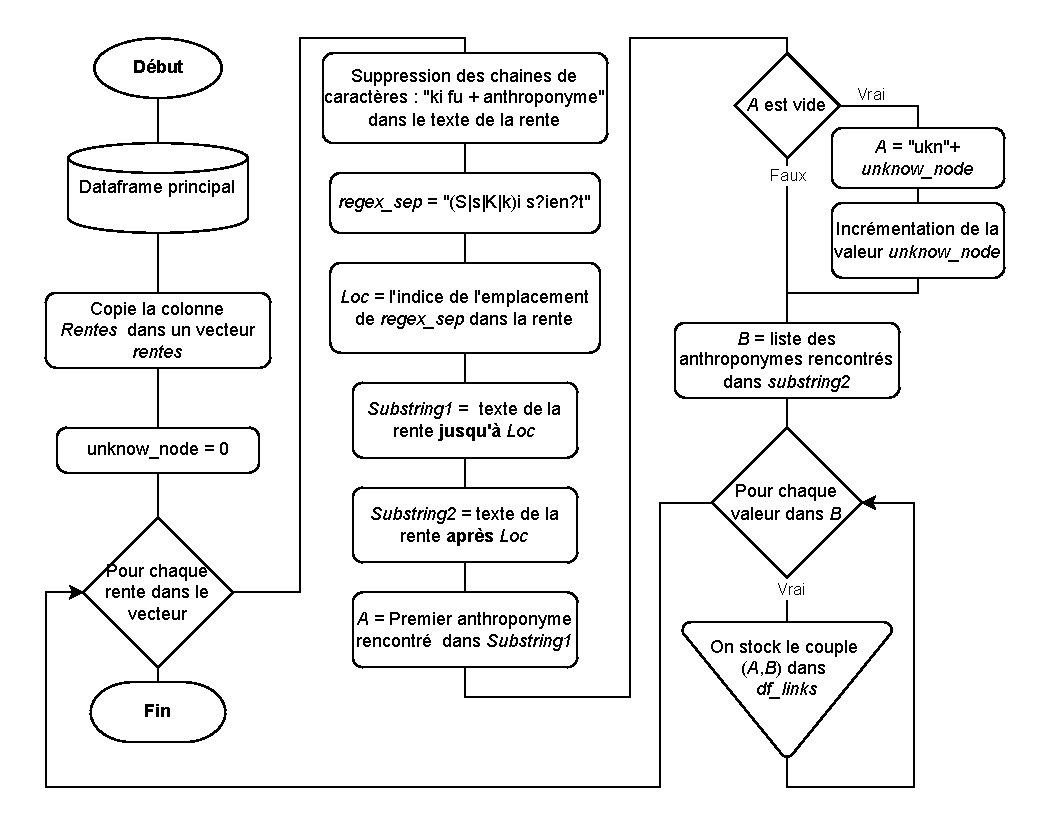
\includegraphics[scale=0.75]{3.Results/Img/rel.drawio.pdf}
    \caption{Organigramme de l'algorithme d'extraction des relations}
    \label{schemaRelations}
\end{figure}

 \begin{figure} % insère une figure ici (h = "here")
    \centering
    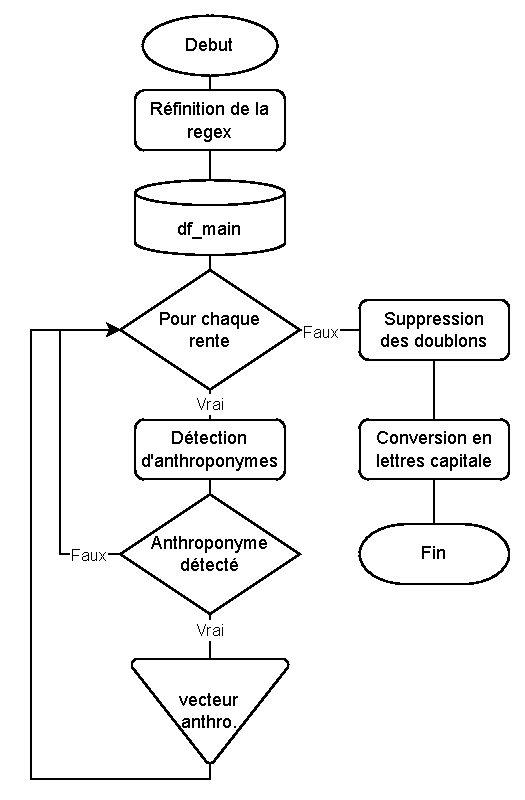
\includegraphics[scale=0.75]{3.Results/Img/clean_df_links.drawio.pdf}
    \caption{Organigramme de l'algorithme de nettoyage des paires}
    \label{schemaNettoyageRelations}
\end{figure}
 
 À la fin de cette opération, nous récupérons  un tableau de données contenant 499 couples. Parmi ceux-ci, nous observons 14 valeurs \textit{ukn} distinctes, affectant un total de 30 couples.

\subsection{Lever l'inconnue des valeurs manquantes}
Cependant, ces valeurs inconnues ne sont pas une fatalité. La commande R suivante nous permet de trouver les lignes dont il est question.
\[ df\_links[str\_detect(df\_links\$To,'ukn'),]\]
 
 Grâce aux anthroponymes connexes à la valeur inconnue, l'agent humain est dans la possibilité de retrouver les valeurs manquantes avec une recherche plein texte depuis le document source. L'analyse de ces valeurs manquantes permet de corriger certains couples qui auraient créé des erreurs dans la modélisation des graphes,  mais elle peut aussi permettre de comprendre les facteurs qui ont engendré cette perte d'information, et amener à leur correction. Le tableau \ref{ukn_node} regroupe les informations récupérées sur les valeurs manquantes après une investigation manuelle. Sur les 15 valeurs inconnues, 10 peuvent être corrigées. Nous constatons aussi que, à l'exception du \textit{Ukn11}, toutes proviennent d'irrégularités du document source. Dans une grande partie de ces cas, l'irrégularité fait que l'expression régulière ne détecte pas l'anthroponyme (comme lorsqu'il y a uniquement un nom de baptême et aucun patronyme), dans l'autre partie des cas, l'individu débiteur n'est pas clairement désigné dans l'énoncé de la rente ou  n'est simplement pas une personne (par exemple : L'ospital des Wés).
\begin{table}
    \centering
    \begin{tabular}{|l|l|l|l|}
\hline	\textbf{Ukn}	&	\textbf{Correspondance}	&	\textbf{Rente}	& \textbf{Raison}		\\
\hline
\hline	Ukn0	&	Lotin	&	5.5	&	Pas de patronyme	\\
\hline	Ukn1	&	Robiert	&	13.7	&	Pas de patronyme	\\
\hline	Ukn2	&	\textit{NA}	&	18.1	&	Pas de débiteur identifié	\\
\hline	Ukn3	&	les 2 sereurs des Lices	&	20.3	&	Sobriquet , qualificatif ou fonction	\\
\hline	Ukn4	&	le prestre des Charteriers	&	32.2	&	Sobriquet, qualificatif ou fonction	\\
\hline	Ukn5	&	Godin	&	44.3	&	Pas de patronyme	\\
\hline	Ukn6	&	\textit{NA}	&	74.12	&	Pas de débiteur identifié	\\
\hline	Ukn7	&	\textit{NA}	&	81.6	&	Pas de débiteur identifié	\\
\hline	Ukn8	&	des Carterier et des Malades	&	95.3	&	Sobriquet , qualificatif ou fonction	\\
\hline	Ukn9	&	Hamiel	&	103.	&	Pas de patronyme	\\
\hline	Ukn10	&	Daniel	&	140.5	&	Pas de patronyme	\\
\hline	Ukn11	&	Mariien de l'Eve	&	150.3	&	Anthroponyme non détecté par la RegEx	\\
\hline	Ukn12	&	Marien	&	151.4	&	Pas de patronyme	\\
\hline	Ukn13	&	L'ospital des Wes	&	206.4	&	N'est pas un anthroponyme	\\
\hline	Ukn14	&	\textit{NA}	&	244.3	&	Pas de débiteur identifié	\\
\hline
    \end{tabular}
    \caption{Valeurs manquantes dans le tableau des relations}
    \label{ukn_node}
\end{table}


\subsection{Corrections supplémentaires}
Les rentes étant classées selon un ordre topographique, il est régulier qu'un même anthroponyme apparaisse dans l'énoncé de deux ou trois rentes successives : une première fois, comme voisin d'un bien arrenté, une seconde fois, comme débiteur de la rente suivante, et une troisième fois, à nouveau comme voisin d'un autre bien arrenté adjacent au sien. Après avoir identifié les individus derrière les valeurs manquantes, il peut donc être également  intéressant de vérifier la rente précédente  et la rente suivante de chacun de ceux-ci ; au besoin, ajouter les relations  au tableau de données. Le tableau \ref{tab:corr_relation} indique les relations qui ont été incorporées au tableau de données après l'analyse manuelle des rentes précédentes et suivantes à celle d'où provenaient les valeurs manquantes.
\begin{table}
    \centering
    \begin{tabular}{|l|c|c|}
    \hline
    \textbf{N° de rente} & \textbf{From} & \textbf{To} \\
    \hline
    \hline	12.6	&	ROBIERT	&	ROBIERT DE FIERIN	\\
    \hline	14.8	&	TENEMENT DES MALADES	&	BAUDE L'ARTISIEN	\\
    \hline	139.4	&	DANIEL	&	JEHAN LE GIERMAIN	\\
    \hline	149.2	&	MARIIEN DE L'EVE	&	PIERON DE HASNON	\\
    \hline	151.4	&	MARIIEN DE L'EVE	&	MARIEN	\\
    \hline	152.5	&	MARIEN	&	MARGOT DE MAGNI	\\
    \hline
    \end{tabular}
    \caption{Relations ajoutées au tableau de données}
    \label{tab:corr_relation}
\end{table}
 
\section{Modélisation des graphes}
\subsection{Modes de représentation}
Il existe différents modes pour la représentation des objets que sont les graphes. Les trois principaux sont :
\begin{itemize}
    \item La liste <<origine/destination>> des liens,
    \item La matrice d'adjacence,
    \item La graphe sous sa forme graphique.
\end{itemize}

Ces trois formes sont équivalentes, dès lors, pour modéliser un graphe sous sa forme graphique, il est possible d'utiliser, soit une liste des liens, soit une matrice d'adjacence. La figure \ref{fig:representation_graphes}\footfullcite[p.5]{beauguitte_graphes_2010} illustre ces trois modes. Dans notre cas, nous utilisons la liste de liens  <<origine/destination>> qui est assemblée lors de la phase \textit{d'extraction des relations}, qui est la méthode la plus conventionnelle.
\begin{figure}
    \centering
    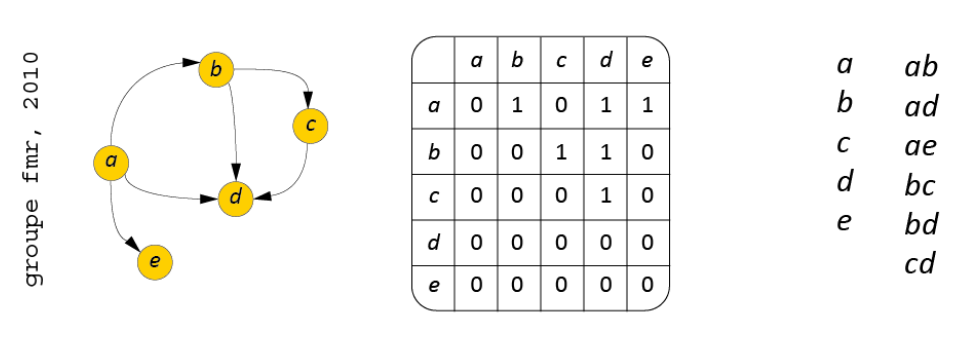
\includegraphics[scale=0.75]{3.Results/Img/mode_de_representation_graphes.png}
    \caption{Trois modes de représentation pour un même objet}
    \label{fig:representation_graphes}
\end{figure}

\subsection{Création de l'objet Igraph et modélisation}
La modélisation des graphes se fait par la fonction  \textit{graph\_from\_data\_frame()}, de la bibliothèque \textit{Igraph}, avec en paramètre le tableau de données \textit{df\_links}.
Cette fonction convertit le tableau de données introduit  en un objet Igraph  reprenant toutes les caractéristiques du graphe. Cet objet peut ensuite être traduit en visualisation en employant la fonction de base \textit{plot()} ou \textit{ggraph()}.

\begin{figure}[h]
    \centering
    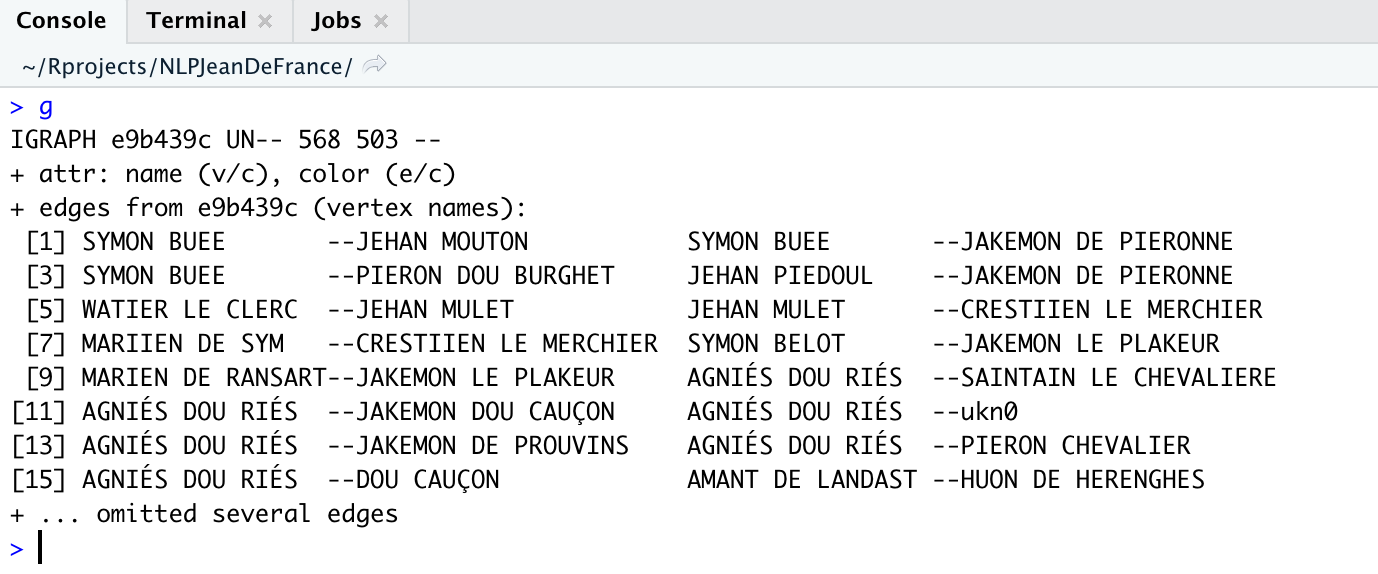
\includegraphics[scale=0.50]{3.Results/Img/igraph_object.png}
    \caption{Objet Igraph convertible en visualisation graphique}
    \label{fig:objetIgraph}
\end{figure}

% premier exemple
Un premier essaie avec les paramètres par défaut, sur un ensemble choisi aléatoirement de cinq rentes successives\footnote{Il s'agit des rentes 19.2 , 20.3, 21.4, 22.1 et 23.2 } nous donne le résultat de la figure  \ref{fig:test_graphe}.

\begin{figure}[h]
    \centering
    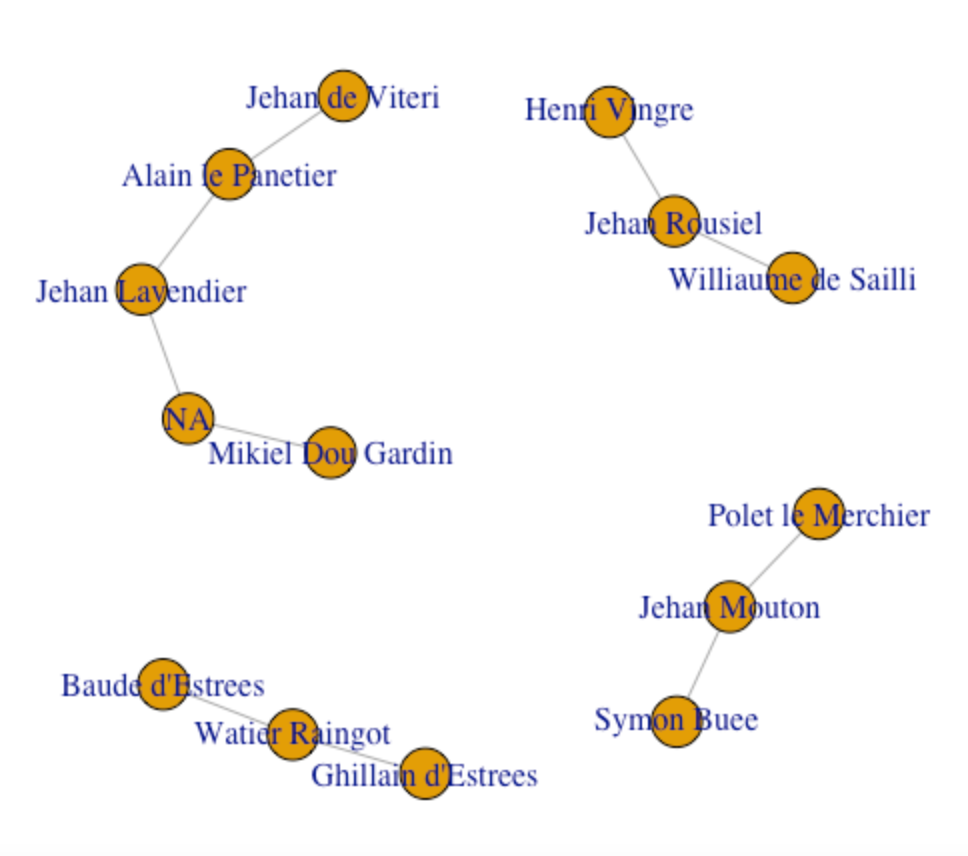
\includegraphics[scale=0.45]{3.Results/Img/graphe_test.png}
    \caption{Graphe des relations mitoyennes, généré sur base des rentes 19.2 à 23.2 }
    \label{fig:test_graphe}
\end{figure}

%modélisation
Lorsque le graphe comprend un nombre important de sommets, comme dans  notre cas, il est plutôt désigné comme \textit{grand graphe} ou comme \textit{grands réseaux}. Cela implique de devoir adapter les paramètres  de la fonction qui modélise le  graphe, sous peine que ce dernier ne devienne illisible par le chevauchement des sommets, des arêtes ou des labels.

Par rapport au premier graphe de la figure \ref{fig:test_graphe}, la taille des sommets a donc été réduite et les labels des sommets ont été supprimés, à l'exception de celui de Jehan de Franche. Également,  une couleur a été affectée à chaque arête en fonction de l'escroete contenant la relation. Pour finir, la spatialisation, c'est-à-dire,  l'algorithme qui définit l'emplacement des sommets dans le plan, est définie par le paramètre \textit{layout}. Pour générer le graphe de la figure  \ref{fig:plot_igraph}, c'est le layout \textit{layout\_nicely} qui a été sélectionné. Ce layout tente de déterminer lui-même la spatialisation la plus appropriée. À ce stade, les sommets sont encore placés de manière non déterministe : chaque appel de la fonction \textit{plot()}  générera un graphe différent, et ce, bien que les paramètres soient inchangés. Cette visualisation nous permet toute foi d'avoir un premier regard  sur la connectivité  des sommets, la longueur des chemins et leur localisation au niveau des escroetes.

\begin{figure}
    \centering
    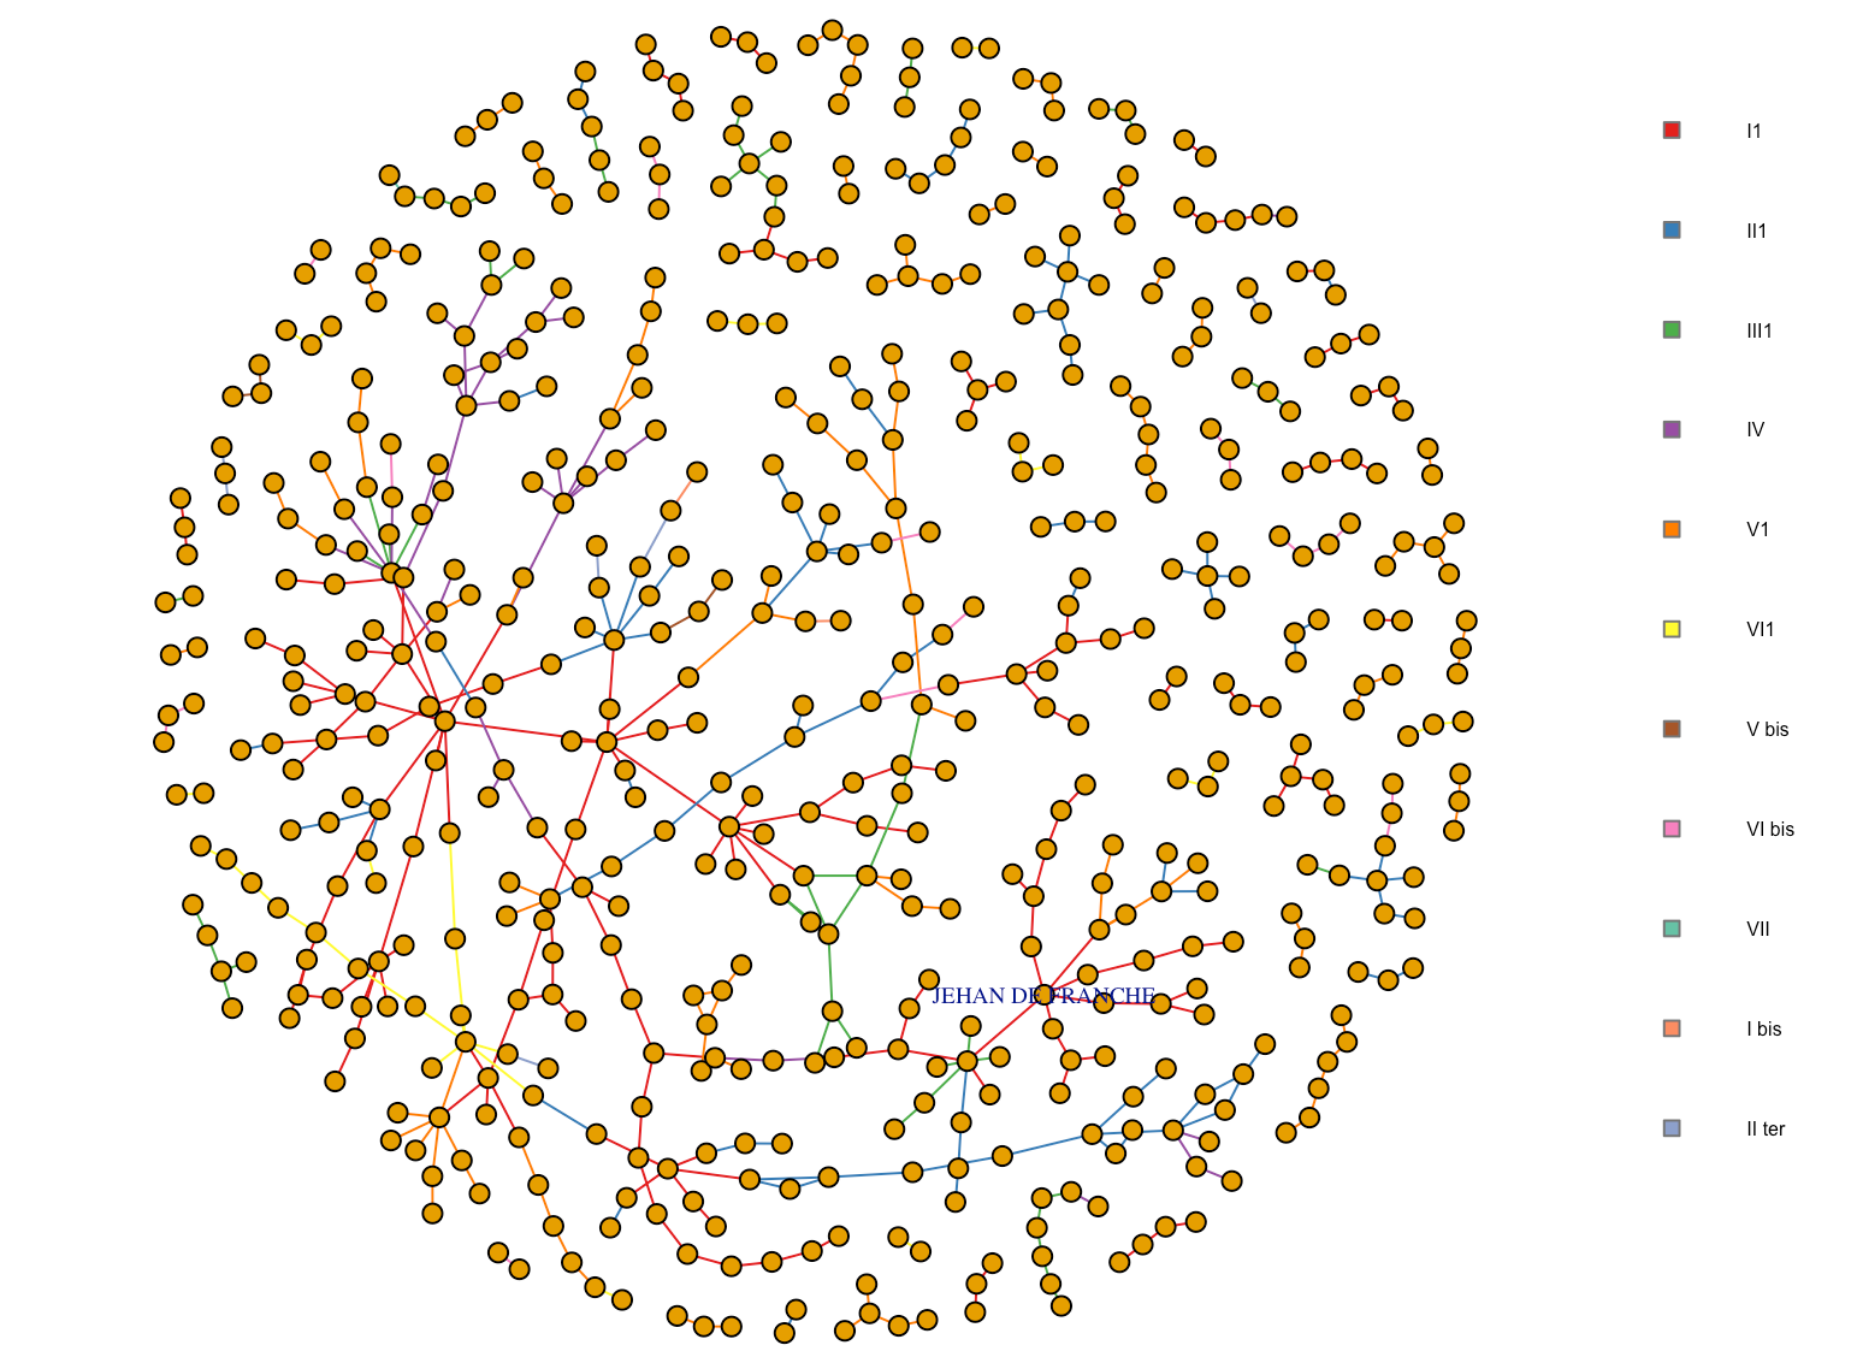
\includegraphics[scale=0.45]{3.Results/Img/plot_igraph.png}
    \caption{Graphe des relations mitoyennes, généré sur base de la fouille de texte automatisée dans le registre de rentes de Jean de France }
    \label{fig:plot_igraph}
\end{figure}

D'autres algorithmes de spatialisation ont été testés, mais aucun ne s'est révélé réellement plus pertinent comme le montre la figure \ref{fig:layout}.

\begin{figure}
    \centering
    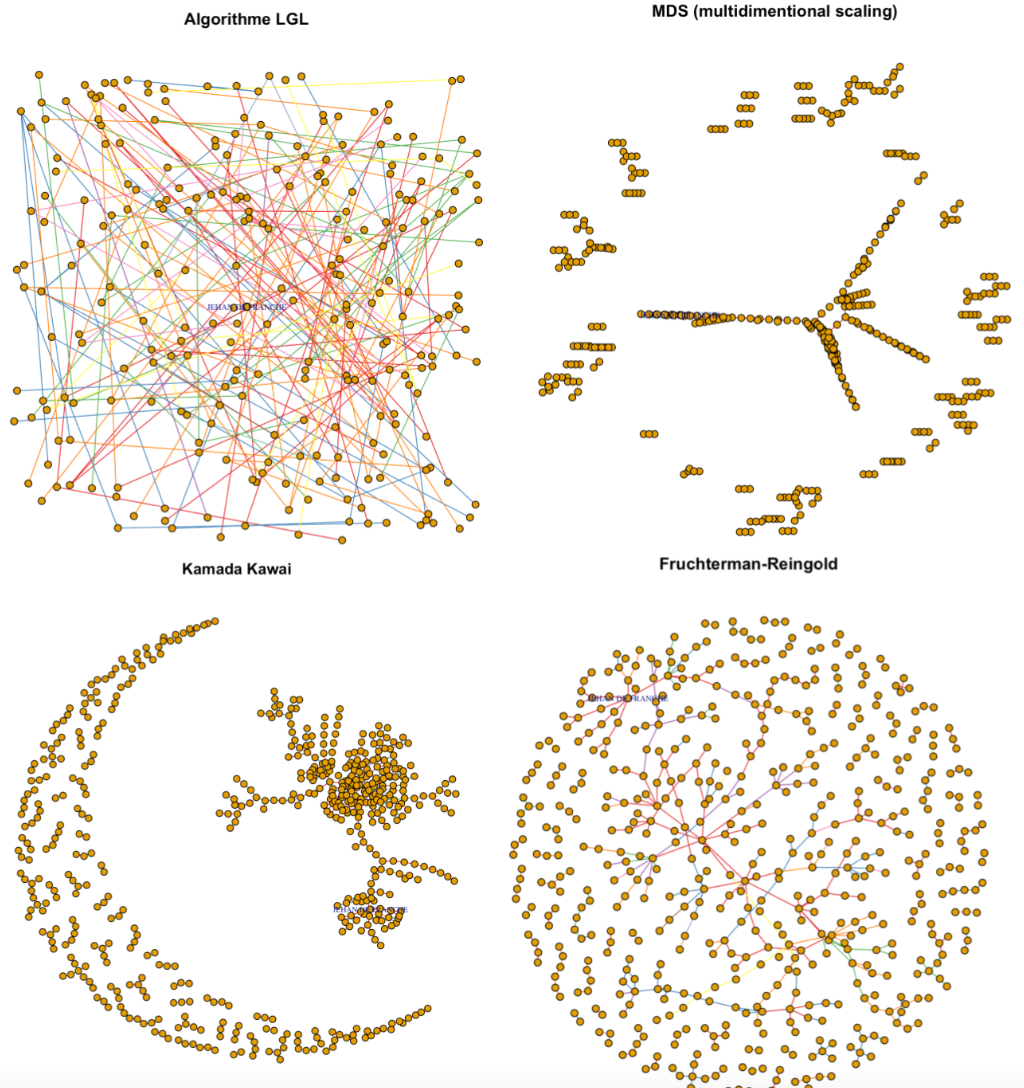
\includegraphics[scale=0.5]{3.Results/Img/layout.png}
    \caption{Différents algorithmes de spatialisation}
    \label{fig:layout}
\end{figure}
